\documentclass[10pt]{myland}

%%%%%%%%%%%%%%%%%%%%%%%%%%%%FILE%%%%%%%%%%%%%%%%%%%%%%%%%%%%%%%%%%%%
\begin{document}
\begin{center}
	{\Large \myhwname} \\
	\vspace{.05in}
    \myname\quad\quarter \\
	\vspace{.05in}
    \today \\
\end{center}
\vspace{.15in} \hrule \vspace{0.5em}%

%%%%% SECTION 1 %%%%%
\begin{enumerate}[label=\textbf{\arabic*.}, listparindent=0.0em, itemsep=1em]
	\item
	Lab 1 contains necessary methods for constructing databases and operators for query plan execution (just reading
	from file in Lab 1 with \texttt{SeqScan}). Key componants implemented are:
	\begin{itemize}
		\item \texttt{Tuple}: this presents a single record (row) in a relation
		\item \texttt{TupleDesc}: this defines the schema of a relation (the number of fields, )
		\item \texttt{Catalog}: this stores information of all relations (tables) currently in the database, including the file, name, and the name of the primary key
		\item \texttt{BufferPool}: this caches the pages recently read by \texttt{DbFile} for good locality performance
		\item \texttt{HeapPage}: this stores the actual data (\texttt{byte} array) stored in a page
		\item \texttt{HeapFile}: this represents a file stored on disk as a collection of \texttt{HeapPage}
		\item \texttt{SeqScan}: this implements sequential scan operator for reading from tuples from \texttt{HeapFile}
	\end{itemize}
    Putting them together, the workflow of a simple reading query is \\
    SQL Query: \texttt{SELECT * FROM EXAMPLE} \\

    Workflow (\texttt{open()}): \\
    \begin{center}
        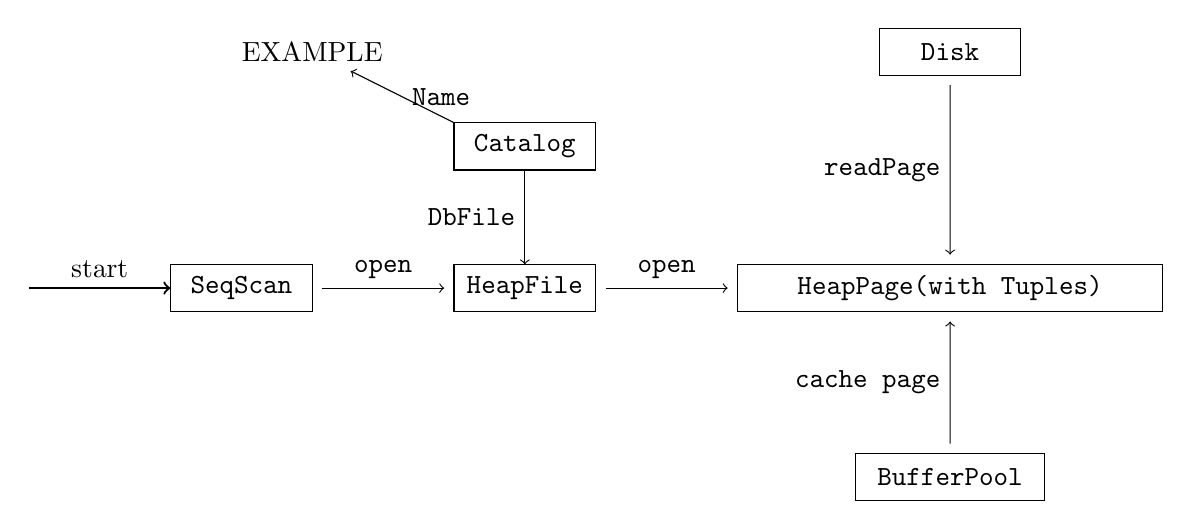
\begin{tikzpicture}[
            scale=.6,
        ]
            \path[->, thick] (-3, -0.5) edge node[midway, above] {start} (0, -0.5);
            \draw[draw=black] (0, 0) rectangle (3, -1) node[midway]  {\texttt{SeqScan}};
            \node (seq) at (3, -0.5) {};
            \draw[draw=black] (6, 0) rectangle (9, -1) node[midway] {\texttt{HeapFile}};
            \node (heapfilel) at (6, -0.5) {};
            \node (heapfiler) at (9, -0.5) {};
            \path[->] (seq) edge node[midway, above] {\texttt{open}} (heapfilel);
            \draw[draw=black] (12, 0) rectangle (21, -1) node[midway] {\texttt{HeapPage(with Tuples)}};
            \node (pagel) at (12, -0.5) {};
            \node (pager) at (21, -0.5) {};
            \node (pageu) at (16.5, 0) {};
            \node (paged) at (16.5, -1) {};
            \path[->] (heapfiler) edge node[midway, above] {\texttt{open}} (pagel);
            \draw[draw=black] (15, 5) rectangle (18, 4) node[midway] {\texttt{Disk}};
            \node (disk) at (16.5, 4) {};
            \path[->] (disk) edge node[midway, left] {\texttt{readPage}} (pageu);
            \draw[draw=black] (14.5, -5) rectangle (18.5, -4) node[midway] {\texttt{BufferPool}};
            \node (buffer) at (16.5, -4) {};
            \path[->] (buffer) edge node[midway, left] {\texttt{cache page}} (paged);
            % catalog
            \draw[draw=black] (6, 3) rectangle (9, 2) node[midway] {\texttt{Catalog}};
            \path[->] (7.5, 2) edge node[midway, left] {\texttt{DbFile}} (7.5, 0);
            \node (name) at (3, 4.5) {EXAMPLE};
            \path[->] (6, 3) edge node[midway, right] {\texttt{Name}} (name);
        \end{tikzpicture}
    \end{center}

    Workflow (\texttt{next()}): \\
    \begin{center}
        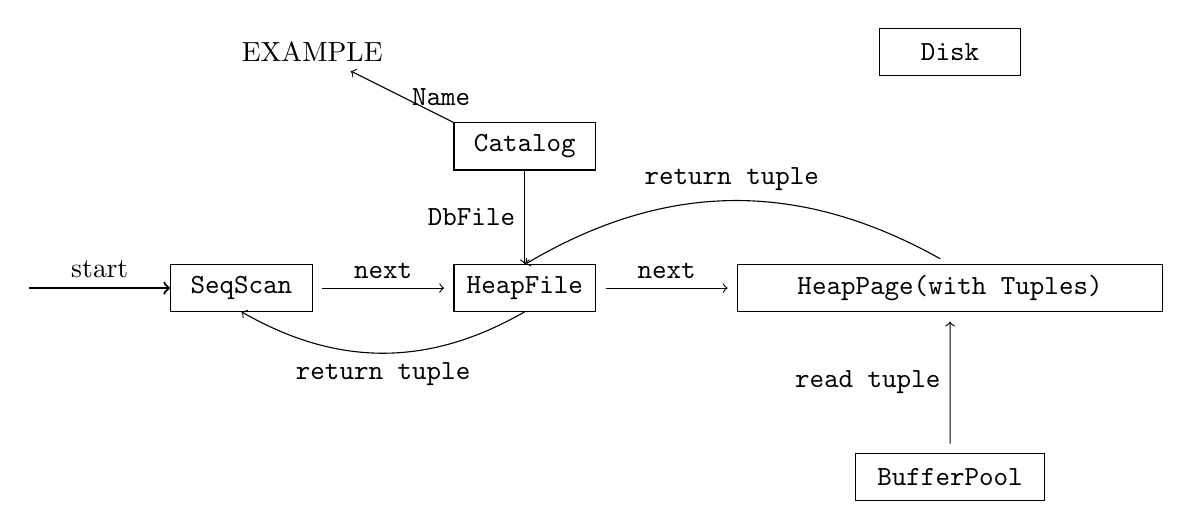
\begin{tikzpicture}[
            scale=.6,
        ]
            \path[->, thick] (-3, -0.5) edge node[midway, above] {start} (0, -0.5);
            \draw[draw=black] (0, 0) rectangle (3, -1) node[midway]  {\texttt{SeqScan}};
            \node (seq) at (3, -0.5) {};
            \draw[draw=black] (6, 0) rectangle (9, -1) node[midway] {\texttt{HeapFile}};
            \node (heapfilel) at (6, -0.5) {};
            \node (heapfiler) at (9, -0.5) {};
            \path[->] (seq) edge node[midway, above] {\texttt{next}} (heapfilel);
            \draw[draw=black] (12, 0) rectangle (21, -1) node[midway] {\texttt{HeapPage(with Tuples)}};
            \node (pagel) at (12, -0.5) {};
            \node (pager) at (21, -0.5) {};
            \node (pageu) at (16.5, 0) {};
            \node (paged) at (16.5, -1) {};
            \path[->] (heapfiler) edge node[midway, above] {\texttt{next}} (pagel);
            \draw[draw=black] (15, 5) rectangle (18, 4) node[midway] {\texttt{Disk}};
            \node (disk) at (16.5, 4) {};
            \draw[draw=black] (14.5, -5) rectangle (18.5, -4) node[midway] {\texttt{BufferPool}};
            \node (buffer) at (16.5, -4) {};
            \path[->] (buffer) edge node[midway, left] {\texttt{read tuple}} (paged);
            \path[->] (pageu) edge [bend right] node[midway, above] {\texttt{return tuple}} (7.5, 0) ;
            \path[->] (7.5, -1) edge [bend left] node[midway, below] {\texttt{return tuple}} (1.5, -1) ;
            \draw[draw=black] (6, 3) rectangle (9, 2) node[midway] {\texttt{Catalog}};
            \path[->] (7.5, 2) edge node[midway, left] {\texttt{DbFile}} (7.5, 0);
            \node (name) at (3, 4.5) {EXAMPLE};
            \path[->] (6, 3) edge node[midway, right] {\texttt{Name}} (name);
        \end{tikzpicture}
    \end{center}

    \item Design decisions: I followed the instructions in README and didn't make extra design decisions.
    \item Extra Unit tests: A unit test for the correctness of \texttt{HeapPage.iterator()} would be nice. My initial
          implementation was wrong because I include the tuples in the empty slot, but the unit tests in \texttt{HeapPageIdTest}
          and \texttt{HeapPageReadTest} did not catch this error. It only showed up when I run \texttt{ScanTest} after
          finishing everything, and it was a little hard to connect the dots back to this method.
    \item Changes to API: I did not make changes to the APIs given.
    \item Missing elements: I believe I finished the entire Lab 1
\end{enumerate}
\end{document}